Consider a hot air balloon carrying a basket with two riders. It is floating at a given altitude. Draw free body diagrams for the following:

\begin{enumerate}
    \item Draw a FBD for the whole system (balloon + basket) using equivalent forces to represent all distributed (body and contact) forces.
    \item Draw an FBD for the basket using equivalent forces to represent all distributed forces.
    \item Draw a FBD for the balloon (not including the basket) using distributed forces.
\end{enumerate}

\begin{solution}\
\begin{center}
    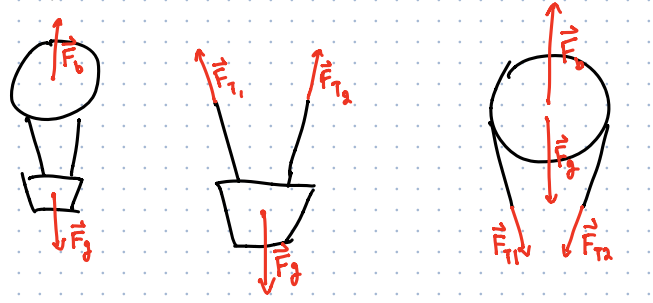
\includegraphics[width=0.75\textwidth]{img/e7p2.png}
\end{center}
\end{solution}